\documentclass[11pt]{article}
\usepackage{amsmath}
\usepackage{pslatex}
\usepackage{natbib}
\usepackage{setspace}
%\usepackage[sc]{mathpazo}
%\usepackage[T1]{fontenc}
\usepackage[margin=1in,pdftex]{geometry}
\setcounter{secnumdepth}{2}
\setcounter{tocdepth}{2}
\usepackage{url}
\usepackage[unicode=true,pdfusetitle,
 bookmarks=true,bookmarksnumbered=true,bookmarksopen=true,bookmarksopenlevel=2,
 breaklinks=false,pdfborder={0 0 1},backref=false,colorlinks=false]{hyperref}
\hypersetup{pdfstartview={XYZ null null 1}}
\usepackage{breakurl}
%\usepackage[authoryear]{natbib}

\newcommand{\quanteda}{\textsf{quanteda}\ }

\usepackage{Sweave}
\begin{document}
\Sconcordance{concordance:quanteda.tex:quanteda.Rnw:%
1 28 1 50 0 1 5 106 1 5 0 9 1 5 0 44 1 3 0 6 1 10 0 20 1 3 0 22 1 2 0 %
14 1 2 0 5 1 5 0 23 1 6 0 11 1 6 0 16 1 5 0 10 1 4 0 8 1 6 0 7 1 5 0 11 %
1 5 0 13 1 5 0 8 1 6 0 8 1 5 0 7 1 6 0 4 1}

%\SweaveOpts{concordance=TRUE}




\begin{Schunk}
\begin{Sinput}
> library(knitr)
> # set global chunk options
> opts_chunk$set(fig.path='figures/minimal-', fig.align='center', fig.show='hold')
> options(replace.assign=TRUE,width=80)
\end{Sinput}
\end{Schunk}

\title{Introduction to the Quantitative Analysis of Textual Data Using
  \quanteda\thanks{This research was supported by the European
    Research Council grant ERC-2011-StG 283794-QUANTESS.  Code
    contributors to the project include Alex Herzog, William Lowe, and
    Kohei Watanabe.}}

\author{Kenneth Benoit and Paul Nulty}

\maketitle

\setlength{\parskip}{1ex}
\setlength{\parindent}{0ex}

\section{Introduction: The Rationale for \quanteda}

\quanteda is an R package designed to simplify the process of
quantitative analysis of text from start to finish, making it possible
to turn texts into a structured corpus, conver this corpus into a
quantitative matrix of features extracted from the texts, and to
perform a variety of quanttative analyses on this matrix.  The object
is inference about the data contained in the texts, whether this means
describing characteristics of the texts, inferring quantities of
interests about the texts of their authors, or determining the tone or
topics contained in the texts.  The emphasis of \quanteda is on
\emph{simplicity}: creating a corpus to manage texts and variables
attached to these texts in a straightforward way, and providing
powerful tools to extract features from this corpus that can be
analyzed using quantitative techniques.

The tools for getting texts into a corpus object include: 
\begin{itemize}
\item loading texts from directories of individual files
\item loading texts ``manually'' by inserting them into a corpus using
  helper functions
\item managing text encodings and conversions from source files into
  corpus texts
\item attaching variables to each text that can be used for grouping,
  reorganizing a corpus, or simply recording additional information to
  supplement quantitative analyses with non-textual data
\item recording meta-data about the sources and creation details for
  the corpus.
\end{itemize}

The tools for working with a corpus include:
\begin{itemize}
\item summarizing the corpus in terms of its language units
\item reshaping the corpus into smaller units or more aggregated units
\item adding to or extracting subsets of a corpus
\item resampling texts of the corpus, for example for use in
  non-parametric bootstrapping of the texts \citep[for an example, see][]{lowebenoitPA2013}
  \item Easy extraction and saving, as a new data frame or corpus, key
    words in context (KWIC)
\end{itemize}

For extracting features from a corpus, \quanteda provides the following tools:
\begin{itemize}
\item extraction of word types
\item extraction of word $n$-grams
\item extraction of dictionary entries from user-defined dictionaries
\item feature selection through
  \begin{itemize}
  \item stemming
  \item random selection
  \item document frequency
  \item word frequency
  \item and a variety of options for cleaning word types, such as
    capitalization and rules for handling punctuation.
  \end{itemize}
\end{itemize}

For analyzing the resulting \emph{document-feature} matrix created
when features are abstracted from a corpus, \quanteda provides:
\begin{itemize}
\item scaling models, such as the Poisson scaling model or Wordscores
\item nonparametric visualization, such as correspondence analysis
\item topic models, such as LDA
\item classifiers, such as Naive Bayes or $k$-nearest neighbour
\item sentiment analysis, using dictionaries
\end{itemize}

\quanteda is hardly unique in providing facilities for working with
text -- the excellent \textsf{tm} package already provides many of the
features we have described.  \quanteda is designed to complement those
packages, as well to simplify the implementation of the
text-to-analysis workflow.  \quanteda corpus structures are simpler
objects than in \textsf{tm}, as are the document-feature matrix
objects from \quanteda, compared to the sparse matrix implementation
found in \textsf{tm}.  However, there is no need to choose only one
package, since we provide translator functions from one matrix or
corpus object to the other in \quanteda.

This vignette is designed to introduce you to \quanteda as well as
provide a tutorial overview of its features.

\section{Installing \quanteda}

The code for the \quanteda package currently resides on
\url{http://github/kbenoit/quanteda}.  From an Internet-connected
computer, you can install the package directly using the
\textsf{devtools} package:

<<<<<<< HEAD
\begin{knitrout}
\definecolor{shadecolor}{rgb}{0.969, 0.969, 0.969}\color{fgcolor}\begin{kframe}
\begin{alltt}
\hlkwd{library}\hlstd{(devtools)}
\hlkwa{if} \hlstd{(}\hlopt{!}\hlkwd{require}\hlstd{(quanteda))} \hlkwd{install_github}\hlstd{(}\hlstr{"quanteda"}\hlstd{,} \hlkwc{username} \hlstd{=} \hlstr{"kbenoit"}\hlstd{)}
\end{alltt}
\end{kframe}
\end{knitrout}


For other branches, for instance if you wish to install the
\texttt{dev} branch (containing work in progress) rather than the
master, you should instead run

\begin{knitrout}
\definecolor{shadecolor}{rgb}{0.969, 0.969, 0.969}\color{fgcolor}\begin{kframe}
\begin{alltt}
\hlkwd{install_github}\hlstd{(}\hlstr{"quanteda"}\hlstd{,} \hlkwc{username} \hlstd{=} \hlstr{"kbenoit"}\hlstd{,} \hlkwc{ref} \hlstd{=} \hlstr{"dev"}\hlstd{)}
\end{alltt}
\end{kframe}
\end{knitrout}




\section{Creating a corpus}

\subsection{Loading Documents into Quanteda}

\subsubsection{From a directory of files}

A very common source of files for creating a corpus will be a set of
text files found on a local (or remote) directory.  To load in a set
of these files, we will load a corpus from a set of text files using
information on attributes of the text that have been conveniently
stored in the text document's filename (separated by underscores).
For example, for our corpus of Irish budget speeches, the filename
\texttt{2010\_BUDGET\_03\_Joan\_Burton\_LAB.txt} tells us the year of
the speech (2010), the type (``BUDGET''), a serial number (03), the
first and last name of the speaker, and a party label (``LAB'' for
Labour).

To load this into a corpus object, we will use the
\texttt{corpusFromFilenames} function, supplying a vector of attribute
labels that correspond with the elements of the filename.

\begin{knitrout}
\definecolor{shadecolor}{rgb}{0.969, 0.969, 0.969}\color{fgcolor}\begin{kframe}
\begin{alltt}
\hlkwd{library}\hlstd{(quanteda)}
\hlstd{textfile} \hlkwb{<-} \hlstr{"https://github.com/kbenoit/quanteda/blob/dev/texts/irishbudgets2010.zip"}
\hlkwd{download.file}\hlstd{(textfile,} \hlkwd{basename}\hlstd{(textfile),} \hlkwc{method} \hlstd{=} \hlstr{"curl"}\hlstd{)}  \hlcom{# download this zipped archive of texts}
\hlcom{# unzip(basename(textfile)) # unzip the file}
\hlstd{attNames} \hlkwb{<-} \hlkwd{c}\hlstd{(}\hlstr{"year"}\hlstd{,} \hlstr{"debate"}\hlstd{,} \hlstr{"number"}\hlstd{,} \hlstr{"firstname"}\hlstd{,} \hlstr{"surname"}\hlstd{,} \hlstr{"party"}\hlstd{)}
\hlcom{# ieBudgets2010 <- corpusFromFilenames(gsub('.zip', '', basename(amicusFile)),}
\hlcom{# c('year', 'debate', 'no', 'fname', 'speaker', 'party'), sep='_')}
\end{alltt}
\end{kframe}
\end{knitrout}


This creates a new quanteda corpus object where each text has been associated values for its attribute types extracted from the filename:

\begin{knitrout}
\definecolor{shadecolor}{rgb}{0.969, 0.969, 0.969}\color{fgcolor}\begin{kframe}
\begin{alltt}
\hlkwd{data}\hlstd{(iebudgets)}
\hlkwd{summary}\hlstd{(iebudgets)}
\end{alltt}
\begin{verbatim}
## Corpus object contains 196 texts.
## 
##                                       Texts Types Tokens Sentences year debate
##        2012_BUDGET_01_Michael_Noonan_FG.txt  1538   6450       294 2012 BUDGET
##       2012_BUDGET_02_Michael_McGrath_FF.txt  1417   6098       307 2012 BUDGET
##        2012_BUDGET_03_Pearse_Doherty_SF.txt  1607   6813       378 2012 BUDGET
##        2012_BUDGET_04_Mick_Wallace_Indp.txt   577   1531        98 2012 BUDGET
##     2012_BUDGET_05_Richard_Barrett_PBPA.txt   577   1820        88 2012 BUDGET
##          2012_BUDGET_06_Shane_Ross_Indp.txt   505   1575        78 2012 BUDGET
##            2012_BUDGET_07_Enda_Kenny_FG.txt  1092   4000       183 2012 BUDGET
##         2012_BUDGET_08_Pat_Rabbitte_LAB.txt  1015   3613       199 2012 BUDGET
##        2012_BUDGET_09_Micheal_Martin_FF.txt  1355   5016       258 2012 BUDGET
##           2012_BUDGET_10_Gerry_Adams_SF.txt  1131   3510       199 2012 BUDGET
##          2012_BUDGET_11_Joe_Higgins_SOC.txt   650   1850        66 2012 BUDGET
##      2012_BUDGET_12_Finian_McGrath_Indp.txt   666   2111       119 2012 BUDGET
##        2012_BUDGET_13_Richard_Bruton_FG.txt   487   1414        56 2012 BUDGET
##         2012_BUDGET_14_Ruairi_Quinn_LAB.txt   462   1545        54 2012 BUDGET
##         2012_BUDGET_15_Ciaran_Cannon_FG.txt   584   1716        73 2012 BUDGET
##           2012_BUDGET_16_Willie_ODea_FF.txt   904   2798       147 2012 BUDGET
##           2012_BUDGET_17_Seamus_Kirk_FF.txt   517   1217        56 2012 BUDGET
##         2012_BUDGET_18_Simon_Coveney_FG.txt   651   2044        86 2012 BUDGET
##          2012_BUDGET_19_James_Reilly_FG.txt   708   2473        97 2012 BUDGET
##       2012_BUDGET_20_Jonathan_OBrien_SF.txt   464   1143        58 2012 BUDGET
##         2012_BUDGET_21_Brian_Stanley_SF.txt   517   1382        72 2012 BUDGET
##      2012_BUDGET_22_Michael_Colreavy_SF.txt   306    652        30 2012 BUDGET
##          2012_BUDGET_23_Dessie_Ellis_SF.txt   319    643        27 2012 BUDGET
##          2012_BUDGET_24_Alan_Shatter_FG.txt  1244   4761       187 2012 BUDGET
##   2012_BUDGET_25_Maureen_OSullivan_Indp.txt   526   1331        65 2012 BUDGET
##       2012_BUDGET_26_John_Halligan_Indp.txt   405    903        46 2012 BUDGET
##        2012_BUDGET_27_Seamus_Healy_WUAG.txt   324    801        53 2012 BUDGET
##      2012_BUDGET_28_Thomas_Pringle_Indp.txt   438    855        46 2012 BUDGET
##          2012_BUDGET_29_Leo_Varadkar_FG.txt   909   3341       161 2012 BUDGET
##           2012_BUDGET_30_Alan_Kelly_LAB.txt   515   1441        68 2012 BUDGET
##          2012_BUDGET_31_Michael_Ring_FG.txt   310    929        61 2012 BUDGET
##         2012_BUDGET_32_Dara_Calleary_FF.txt   685   2168       107 2012 BUDGET
##           2012_BUDGET_33_John_Browne_FF.txt   408   1168        56 2012 BUDGET
##          2012_BUDGET_34_Timmy_Dooley_FF.txt   430   1079        53 2012 BUDGET
##        2012_BUDGET_35_Jimmy_Deenihan_FG.txt   646   2247       100 2012 BUDGET
##           2012_BUDGET_36_Brian_Hayes_FG.txt   430   1199        54 2012 BUDGET
##         2012_BUDGET_37_Peadar_Toibin_SF.txt   537   1393        75 2012 BUDGET
##       2012_BUDGET_38_Sandra_McLellan_SF.txt   520   1373        67 2012 BUDGET
##  2012_BUDGET_39_Padraig_MacLochlainn_SF.txt   392    997        51 2012 BUDGET
##            2012_BUDGET_40_Sean_Crowe_SF.txt   274    563        33 2012 BUDGET
##    2012_BUDGET_41_Frances_Fitzgerald_FG.txt   633   2212       124 2012 BUDGET
##        2012_BUDGET_42_Jan_OSullivan_LAB.txt   550   1618        66 2012 BUDGET
##            2012_BUDGET_43_John_Perry_FG.txt   406   1016        45 2012 BUDGET
##       2012_BUDGET_44_John_McGuinness_FF.txt   498   1650        98 2012 BUDGET
##           2012_BUDGET_45_Eamon_OCuiv_FF.txt   703   2502       123 2012 BUDGET
##       2012_BUDGET_46_Olivia_Mitchell_FG.txt   388    886        49 2012 BUDGET
##        2012_BUDGET_47_Jerry_Buttimer_FG.txt   418    977        50 2012 BUDGET
##        2012_BUDGET_48_Bernard_Durkan_FG.txt   399   1213        62 2012 BUDGET
##             2012_BUDGET_49_Tom_Barry_FG.txt   436   1135        70 2012 BUDGET
##         2012_BUDGET_50_Tom_Fleming_Indp.txt   427   1036        56 2012 BUDGET
##      2012_BUDGET_51_Mattie_McGrath_Indp.txt   554   1472       109 2012 BUDGET
##       2012_BUDGET_52_Luke_Flanagan_Indp.txt   558   1697        93 2012 BUDGET
##     2012_BUDGET_53_Dominic_Hannigan_LAB.txt   335    887        51 2012 BUDGET
##        2012_BUDGET_54_Arthur_Spring_LAB.txt   291    641        32 2012 BUDGET
##         2011_BUDGET_01_Brian_Lenihan_FF.txt  1537   7094       371 2011 BUDGET
##        2011_BUDGET_02_Michael_Noonan_FG.txt  1110   4275       227 2011 BUDGET
##          2011_BUDGET_03_Joan_Burton_LAB.txt  1262   4654       254 2011 BUDGET
##        2011_BUDGET_04_Pearse_Doherty_SF.txt  1337   5941       326 2011 BUDGET
##           2011_BUDGET_05_Brian_Cowen_FF.txt  1506   6870       334 2011 BUDGET
##            2011_BUDGET_06_Enda_Kenny_FG.txt  1154   4418       204 2011 BUDGET
##        2011_BUDGET_07_Eamon_Gilmore_LAB.txt  1172   4613       218 2011 BUDGET
##       2011_BUDGET_08_Brendan_Howlin_LAB.txt   463   1163        53 2011 BUDGET
##       2011_BUDGET_09_John_Gormley_Green.txt  1022   3755       181 2011 BUDGET
##   2011_BUDGET_10_Caoimhghin_OCaolain_SF.txt  1438   5282       282 2011 BUDGET
##         2011_BUDGET_11_Eamon_Ryan_Green.txt   513   1629        67 2011 BUDGET
##        2011_BUDGET_12_Micheal_Martin_FF.txt   553   1607        73 2011 BUDGET
##      2011_BUDGET_13_Michael_Finneran_FF.txt   442   1108        48 2011 BUDGET
##          2011_BUDGET_14_James_Reilly_FG.txt   420   1021        65 2011 BUDGET
##          2011_BUDGET_15_Fergus_ODowd_FG.txt   454   1128        72 2011 BUDGET
##       2011_BUDGET_16_Catherine_Byrne_FG.txt   461   1173        62 2011 BUDGET
##        2011_BUDGET_17_Bernard_Durkan_FG.txt   365    895        44 2011 BUDGET
##         2011_BUDGET_18_Brendan_Smith_FF.txt   723   2368       103 2011 BUDGET
##          2011_BUDGET_19_Johnny_Brady_FF.txt   268    563        26 2011 BUDGET
##          2011_BUDGET_20_Batt_OKeeffe_FF.txt   485   1357        67 2011 BUDGET
##          2011_BUDGET_21_Michael_Ring_FG.txt   269    632        40 2011 BUDGET
##         2011_BUDGET_22_Simon_Coveney_FG.txt   381   1009        48 2011 BUDGET
##         2011_BUDGET_23_Deirdre_Clune_FG.txt   274    596        28 2011 BUDGET
##            2011_BUDGET_24_Phil_Hogan_FG.txt   280    602        21 2011 BUDGET
##        2011_BUDGET_25_Jimmy_Deenihan_FG.txt   310    676        40 2011 BUDGET
##          2011_BUDGET_26_Sean_Barrett_FG.txt   337    745        49 2011 BUDGET
##             2011_BUDGET_27_Pat_Carey_FF.txt   438   1279        59 2011 BUDGET
##         2011_BUDGET_28_Mary_White_Green.txt   526   1426        59 2011 BUDGET
##       2011_BUDGET_29_Martin_Mansergh_FF.txt   438   1013        36 2011 BUDGET
##         2011_BUDGET_30_Pat_Rabbitte_LAB.txt   534   1514        64 2011 BUDGET
##      2011_BUDGET_31_Michael_Higgins_LAB.txt   546   1341        62 2011 BUDGET
##       2011_BUDGET_32_Kathleen_Lynch_LAB.txt   277    715        46 2011 BUDGET
##          2011_BUDGET_33_Mary_Hanafin_FF.txt   471   1335        63 2011 BUDGET
##        2011_BUDGET_34_Billy_Kelleher_FF.txt   461   1332        59 2011 BUDGET
##      2011_BUDGET_35_Finian_McGrath_Indp.txt   296    714        36 2011 BUDGET
##   2011_BUDGET_36_Maureen_OSullivan_Indp.txt   292    618        21 2011 BUDGET
##      2011_BUDGET_37_Mattie_McGrath_Indp.txt   216    490        25 2011 BUDGET
##         2010_BUDGET_01_Brian_Lenihan_FF.txt  1655   7799       390 2010 BUDGET
##        2010_BUDGET_02_Richard_Bruton_FG.txt   956   4058       222 2010 BUDGET
##          2010_BUDGET_03_Joan_Burton_LAB.txt  1485   5770       329 2010 BUDGET
##         2010_BUDGET_04_Arthur_Morgan_SF.txt  1463   6481       349 2010 BUDGET
##           2010_BUDGET_05_Brian_Cowen_FF.txt  1473   5880       262 2010 BUDGET
##            2010_BUDGET_06_Enda_Kenny_FG.txt  1066   3875       161 2010 BUDGET
##       2010_BUDGET_07_Kieran_ODonnell_FG.txt   614   2066       141 2010 BUDGET
##        2010_BUDGET_08_Eamon_Gilmore_LAB.txt  1098   3800       208 2010 BUDGET
##      2010_BUDGET_09_Michael_Higgins_LAB.txt   447   1136        49 2010 BUDGET
##  no      fname      speaker party
##  01    Michael       Noonan    FG
##  02    Michael      McGrath    FF
##  03     Pearse      Doherty    SF
##  04       Mick      Wallace  Indp
##  05    Richard      Barrett  PBPA
##  06      Shane         Ross  Indp
##  07       Enda        Kenny    FG
##  08        Pat     Rabbitte   LAB
##  09    Micheal       Martin    FF
##  10      Gerry        Adams    SF
##  11        Joe      Higgins   SOC
##  12     Finian      McGrath  Indp
##  13    Richard       Bruton    FG
##  14     Ruairi        Quinn   LAB
##  15     Ciaran       Cannon    FG
##  16     Willie         ODea    FF
##  17     Seamus         Kirk    FF
##  18      Simon      Coveney    FG
##  19      James       Reilly    FG
##  20   Jonathan       OBrien    SF
##  21      Brian      Stanley    SF
##  22    Michael     Colreavy    SF
##  23     Dessie        Ellis    SF
##  24       Alan      Shatter    FG
##  25    Maureen    OSullivan  Indp
##  26       John     Halligan  Indp
##  27     Seamus        Healy  WUAG
##  28     Thomas      Pringle  Indp
##  29        Leo     Varadkar    FG
##  30       Alan        Kelly   LAB
##  31    Michael         Ring    FG
##  32       Dara     Calleary    FF
##  33       John       Browne    FF
##  34      Timmy       Dooley    FF
##  35      Jimmy     Deenihan    FG
##  36      Brian        Hayes    FG
##  37     Peadar       Toibin    SF
##  38     Sandra     McLellan    SF
##  39    Padraig MacLochlainn    SF
##  40       Sean        Crowe    SF
##  41    Frances   Fitzgerald    FG
##  42        Jan    OSullivan   LAB
##  43       John        Perry    FG
##  44       John   McGuinness    FF
##  45      Eamon        OCuiv    FF
##  46     Olivia     Mitchell    FG
##  47      Jerry     Buttimer    FG
##  48    Bernard       Durkan    FG
##  49        Tom        Barry    FG
##  50        Tom      Fleming  Indp
##  51     Mattie      McGrath  Indp
##  52       Luke     Flanagan  Indp
##  53    Dominic     Hannigan   LAB
##  54     Arthur       Spring   LAB
##  01      Brian      Lenihan    FF
##  02    Michael       Noonan    FG
##  03       Joan       Burton   LAB
##  04     Pearse      Doherty    SF
##  05      Brian        Cowen    FF
##  06       Enda        Kenny    FG
##  07      Eamon      Gilmore   LAB
##  08    Brendan       Howlin   LAB
##  09       John      Gormley Green
##  10 Caoimhghin     OCaolain    SF
##  11      Eamon         Ryan Green
##  12    Micheal       Martin    FF
##  13    Michael     Finneran    FF
##  14      James       Reilly    FG
##  15     Fergus        ODowd    FG
##  16  Catherine        Byrne    FG
##  17    Bernard       Durkan    FG
##  18    Brendan        Smith    FF
##  19     Johnny        Brady    FF
##  20       Batt      OKeeffe    FF
##  21    Michael         Ring    FG
##  22      Simon      Coveney    FG
##  23    Deirdre        Clune    FG
##  24       Phil        Hogan    FG
##  25      Jimmy     Deenihan    FG
##  26       Sean      Barrett    FG
##  27        Pat        Carey    FF
##  28       Mary        White Green
##  29     Martin     Mansergh    FF
##  30        Pat     Rabbitte   LAB
##  31    Michael      Higgins   LAB
##  32   Kathleen        Lynch   LAB
##  33       Mary      Hanafin    FF
##  34      Billy     Kelleher    FF
##  35     Finian      McGrath  Indp
##  36    Maureen    OSullivan  Indp
##  37     Mattie      McGrath  Indp
##  01      Brian      Lenihan    FF
##  02    Richard       Bruton    FG
##  03       Joan       Burton   LAB
##  04     Arthur       Morgan    SF
##  05      Brian        Cowen    FF
##  06       Enda        Kenny    FG
##  07     Kieran     ODonnell    FG
##  08      Eamon      Gilmore   LAB
##  09    Michael      Higgins   LAB
## 
## Source:  /home/paul/* on x86_64 by paul.
## Created: Wed Nov 28 16:49:22 2012.
## Notes:   NA.
\end{verbatim}
\end{kframe}
\end{knitrout}


\subsubsection{From a vector of texts}


\subsection{Adding Information to a corpus}

\subsubsection{Adding new texts}

\subsubsection{Adding new text attributes}


\subsection{Translating a \quanteda corpus into other formats}

\subsubsection{Importing from QDAMiner}

\subsubsection{Importing to and exporting from \textsf{tm}}


\section{Manipulating a corpus}


\section{Extracting Features}


\section{Analyzing a document-feature matrix}





% \singlespacing
\bibliographystyle{apsr}
\bibliography{../../bibliographies/QUANTESS}

\end{document}


In order to perform statistical analysis such as document scaling, we must extract a matrix containing the frequency of each word type from in document. In quanteda, we use the dfm function to produce such a matrix. \footnote{dfm stands for document-feature matrix --- we say `feature' instead of word, as it is sometimes useful to represent documents by features other than their word frequency.}

\begin{knitrout}
\definecolor{shadecolor}{rgb}{0.969, 0.969, 0.969}\color{fgcolor}\begin{kframe}
\begin{alltt}
\hlstd{docMat} \hlkwb{<-} \hlkwd{dfm}\hlstd{(iebudgets)}
\end{alltt}
\begin{verbatim}
## Creating dfm: ... done.
\end{verbatim}
\begin{alltt}
\hlstd{docMat[}\hlnum{1}\hlopt{:}\hlnum{5}\hlstd{,} \hlnum{1}\hlopt{:}\hlnum{5}\hlstd{]}
\end{alltt}
\begin{verbatim}
##                                       words
## docs                                     <U+00A3>   <U+00B0>   <U+00BC>   <U+00BD>
##   2008_BUDGET_01_Brian_Cowen_FF.txt           0        0        1        2
##   2008_BUDGET_02_Richard_Bruton_FG.txt        0        0        0        0
##   2008_BUDGET_03_Joan_Burton_LAB.txt          0        0        0        0
##   2008_BUDGET_04_Arthur_Morgan_SF.txt         0        0        0        0
##   2008_BUDGET_05_Bertie_Ahern_FF.txt          0        0        0        0
##                                       words
## docs                                     <U+00BE>
##   2008_BUDGET_01_Brian_Cowen_FF.txt           1
##   2008_BUDGET_02_Richard_Bruton_FG.txt        0
##   2008_BUDGET_03_Joan_Burton_LAB.txt          0
##   2008_BUDGET_04_Arthur_Morgan_SF.txt         0
##   2008_BUDGET_05_Bertie_Ahern_FF.txt          0
\end{verbatim}
\end{kframe}
\end{knitrout}


We can now score and plot the documents using a statistical scaling technique, for example correspondence analysis.

\begin{knitrout}
\definecolor{shadecolor}{rgb}{0.969, 0.969, 0.969}\color{fgcolor}\begin{kframe}
\begin{alltt}
\hlkwd{library}\hlstd{(ca)}
\hlstd{model} \hlkwb{<-} \hlkwd{ca}\hlstd{(}\hlkwd{t}\hlstd{(docMat),} \hlkwc{nd} \hlstd{=} \hlnum{1}\hlstd{)}
\hlkwd{dotchart}\hlstd{(model}\hlopt{$}\hlstd{colcoord[}\hlkwd{order}\hlstd{(model}\hlopt{$}\hlstd{colcoord[,} \hlnum{1}\hlstd{]),} \hlnum{1}\hlstd{],} \hlkwc{labels} \hlstd{= model}\hlopt{$}\hlstd{colnames[}\hlkwd{order}\hlstd{(model}\hlopt{$}\hlstd{colcoord[,}
    \hlnum{1}\hlstd{])])}
\end{alltt}
\end{kframe}

{\centering 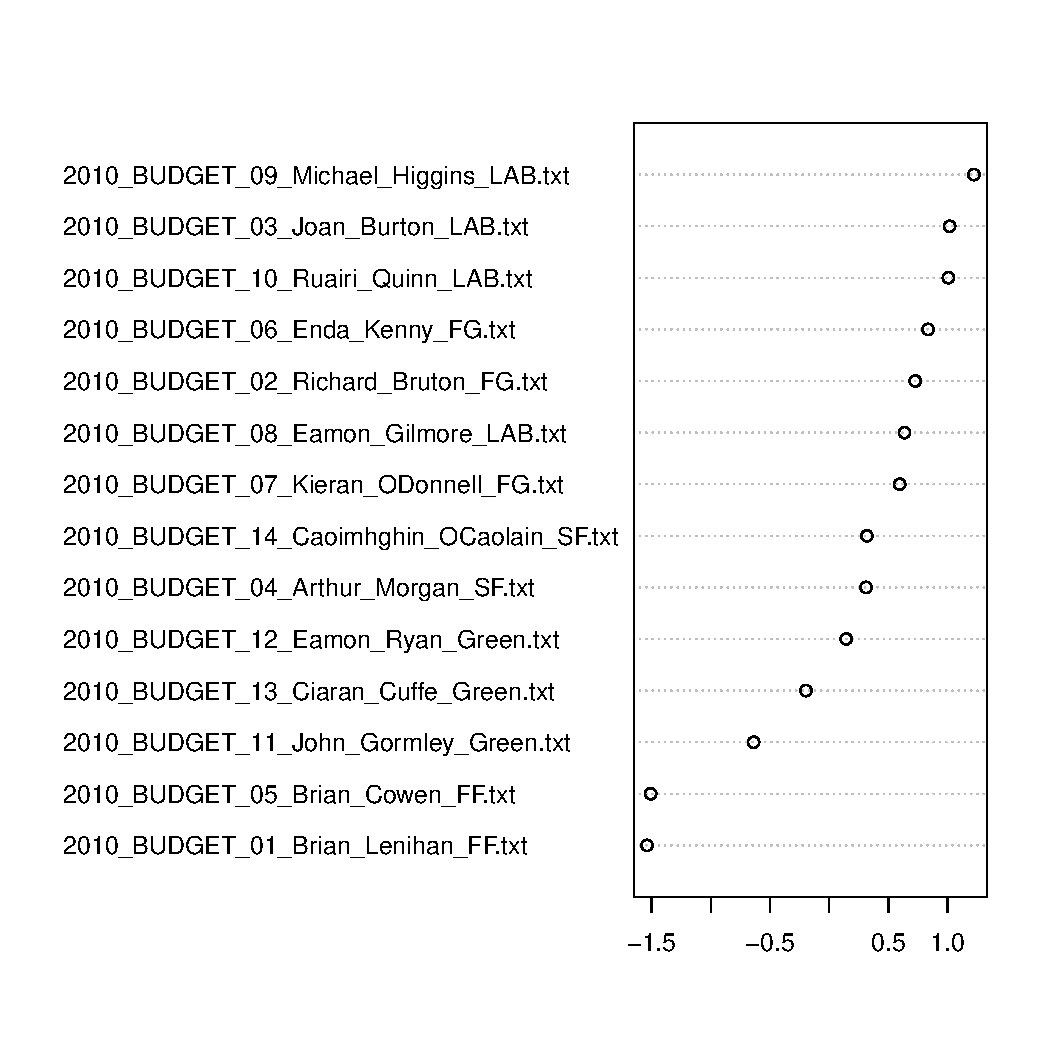
\includegraphics[width=\maxwidth]{figures/minimal-unnamed-chunk-6} 

}



\end{knitrout}


This plot indicates the position
of each of the documents. We can group documents by their attribute values when creating the word-frequency matrix: 

\begin{knitrout}
\definecolor{shadecolor}{rgb}{0.969, 0.969, 0.969}\color{fgcolor}\begin{kframe}
\begin{alltt}
\hlstd{partyMat} \hlkwb{<-} \hlkwd{dfm}\hlstd{(ieBudgets,} \hlkwc{group} \hlstd{=} \hlstr{"party"}\hlstd{)}
\end{alltt}
\begin{verbatim}
## Creating dfm: ... aggregating by group: party...complete ... done.
\end{verbatim}
\begin{alltt}
\hlstd{partyMat[,} \hlnum{1}\hlopt{:}\hlnum{5}\hlstd{]}
\end{alltt}
\begin{verbatim}
##        words
## docs    <c3><89>ireann <c3><93> <e2><80><93>sure <e2><80><94> <e2><80><99>flu
##   FF                 0        0                0            5               0
##   FG                 0        0                1            9               1
##   Green              0        1                0           23               0
##   LAB                1        0                0            9               0
##   SF                 2        0                0            4               0
\end{verbatim}
\end{kframe}
\end{knitrout}


which allows us to scale according to a particular party or year, for example:

\begin{knitrout}
\definecolor{shadecolor}{rgb}{0.969, 0.969, 0.969}\color{fgcolor}\begin{kframe}
\begin{alltt}
\hlstd{partyModel} \hlkwb{<-} \hlkwd{ca}\hlstd{(}\hlkwd{t}\hlstd{(partyMat),} \hlkwc{nd} \hlstd{=} \hlnum{1}\hlstd{)}
\hlkwd{dotchart}\hlstd{(partyModel}\hlopt{$}\hlstd{colcoord[}\hlkwd{order}\hlstd{(partyModel}\hlopt{$}\hlstd{colcoord[,} \hlnum{1}\hlstd{]),} \hlnum{1}\hlstd{],} \hlkwc{labels} \hlstd{= partyModel}\hlopt{$}\hlstd{colnames[}\hlkwd{order}\hlstd{(partyModel}\hlopt{$}\hlstd{colcoord[,}
    \hlnum{1}\hlstd{])])}
\end{alltt}
\end{kframe}

{\centering 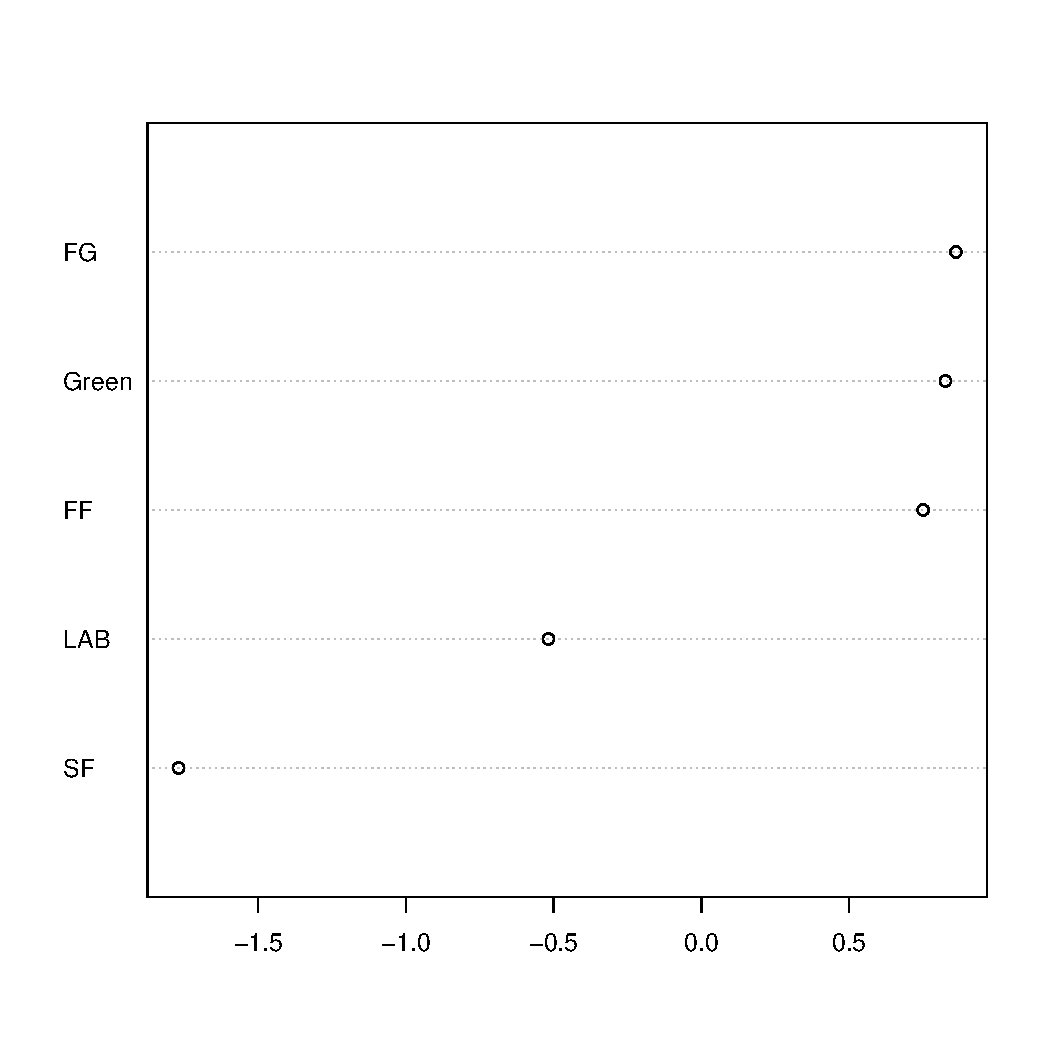
\includegraphics[width=\maxwidth]{figures/minimal-unnamed-chunk-8} 

}



\end{knitrout}


=======
>>>>>>> 304330e5366a2c59f63041efbb1b458948968ddf
